\section{Stand der Forschung und Technik}
Durch die gestiegene Rechenleistung der heutigen Computer ist auch die anwendungshäufigkeit von Genetischen Algorithmen deutlich gestiegen. Es werden nicht nur neue Ansätze erforscht, sondern auch kleiner Anwendungen entwickelt, die nicht nur im IT-Bereich ihre anwendungen finden.

\subsection{Deep Mind}
Den größten Fortschitt der letzen Jahre verzeichnete Googles Deepmind. Deepmind setzt dabei auch auf einen Populations bassierenden Algorithmus, welcher auf den Genetischen Algorithmen aufbaut. Goolge nutz ihre PopulationBasedTraining vorallem im Bereich der Künstlichen Inteligzenz. So konnten sie bei verschiedene Künstlichen Neuronalen Netzen wie AlphaGo(Go)\cite{alphago} und AlphaStar(Starcraft2)\cite{alphastar} deutliche verbesserungen durch das PBT erreichen. Das PBT wird nicht nur für Brett- bzw. Computer-spiele genutzt. Sondern auch für Anwendungen im Bereich des autonomen Fahrens. Dort wurde in zusammenarbeit mit der Google-Tochter Waymo eine deutliche Verbesserung der xxxgesamt Leistungxxx ausgearbeitet. 

\subsection{PopulationBasedTraining}
PBT ist eine weiter entwicklung der klassischen Grid- und Randomsearch und wird von den Genetischen Grundlagen stark beinflusst. PBT ist wie Ga ein Populations bassierender such algorithmus es werden hier auch weiter methoden wie survival of the Fitest und Muation übernommen. Desweitern wurde ein online anpassung der Hyperparameter wärend des Trainings implementiert. Durch dieses Feature, wird viel Rechenleistung eingespaart bzw. das berechnen der Hyperparameter stark beschleunigt. \cite{pbt}

\iffalse
Dies ist zusehen daran das PBT auch eine Population verwendet, auch werden hier die übernahmme des Fitesten und Muationen verwendet. Zudem ist das Training Asynchron und Parallel möglich.
Desweitern wurde ein online anpassung der Hyperparameter wärend des Trainings implementiert. Durch dieses Feature, wird viel Rechenleistung eingespaart bzw. das berechnen der Hyperparameter stark beschleunigt. \cite{pbt}


Sie verwenden Algorithem die dem GA Sehr ähnlich(weiter entwickelt) ist und zwar das Population bassierende Training (eng. Poulation Based Training short PBT). Sie benutzen PBT auch zum anpassen von Hyperparametern speziel für ihre Reinforcment Learning Models. Deep Minds Variante des GA ist sehr viel komplexer. 
Sie haben ein Online-Learn verfahren in welchem sie die Hyperparameter während des Trainings anpassen können, dies ist durch einen einen Server auf dem die daten gespeichert sind möglich. Dieser gibt ihnen auch die möglichkeit Asynchron und Parallel zu arbeiten. Im Durschnitt kontne sie ihre Ergebnisse noch einmal um bis zu 5 Prozent verbessern. 
\fi

\subsection{Software Testing with Ga}
Die Softwarebewertung spielt eine entscheidende Rolle im Lebenszyklus eines Software-Produktionssystems. Die Erzeugung geeigneter Daten zum Testen des Verhaltens der Software ist Gegenstand vieler Forschungen im Software-Engineering. In diesem Beitrag wird die Qualitätskontrolle mit Kriterien zur Abdeckung von Anwendungspfaden betrachtet und ein neues Verfahren auf der Grundlage eines genetischen Algorithmus zur Erzeugung optimaler Testdaten vorgeschlagen. 
\cite{Keshavarz}


\subsection{Travelling Salesman Problem}
Einer der bekanntesten anwendungen für GA ist das Travelling Salesman Problem, in welchem die kürzeste Route beim Austragen von Briefen für einen Postboten berechnet werden soll. Es ist ein Optimales Problem zum Lösen für GA, durch die zurückgelegte steckte kann leichte eine Fitnessfunktion aufgestellt werden. Desweitern wird der Suchbereich mit jedem auszutragenden Brief um einen Expotonenten größer. Und ist somit für gänige Algorothmen nur mit sehr viel Rechnleistung zu bewältigen.

 Doch je mehr Briefe der Postbote austragen soll umso mehr Variablen gibt es, sprich es wird wesentlich schwerer für ein fest geschrieben (eng. Hardcoded) Algorithmus den kürzesten weg zu finden. Für den Ga ist dies kein Problem da mit der richtigen Fitnessfunktion eine einfacher Rückgabewert der Funktion zu bekommen ist. Dementsprechend kann die Route einfach optimiert werden.

\subsection{Temperatur Schätzungen}
--Fällt weg-- wegen GP 
Es gibt auch Forschungen zur berechnung von Temperaturverläufen der Erde \cite{Stanislawska1}. Vom gleichen Author gibt es auch eine abschätzungen von Wärmeflusses zwischen Athmosphäre und Meereies in Polarregeionen \cite{Stanislawska,2}. All diese Vorraussagen wurden mithilfe von Genetischen Programming ausgerechnet. 

In dem die Aufzeichnungen der Temperaturverläufe als Trainingsdaten verwendet werden konnten Lösungen gefunden werden, welche den rellen daten sehr nahe kommen.

\subsection{Generativ Design}
Heute gibt es in viele Computer-aided design(CAD) Programme in welchen es implementierungen von Generativen Design Werkzeugen gibt. In dennen über Iterationen neue mögliche Designs berechnet werden deis passiert auch auf Basis der Genetischen Evolution. Sie bauen nicht auf den Genetischen Algorithmen auf sind aber nahe verwante und sollten nicht unterschätzt werden. 
Mit ihnen ist es möglich Bionische Stukturen für addetive Vertigung zu designen. Und sie speziell auf die Anwendung anpassen. So kann aus einem einfachen Frästeil ein wesentlich Leichtes und Material spaarenderes Model entwickelt werden.

\noindent%
\begin{figure}[H]
  \centering  
  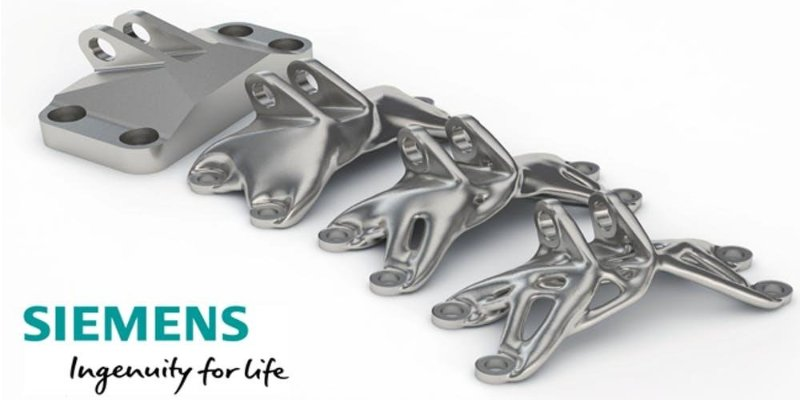
\includegraphics[scale=0.3]{img/Additive.png}
  \caption{Additives Design über mehrer Iterationen}
  \label{fig:Ablauf_kurz}
\end{figure}

\paragraph{NASA - Antenne}
DIe Nasa hat 2006 eine Weltraumantenne mit hilfe evolutionären Algorithmen entwickelt. Die Entwicklung der Antenne von hand ist sehr zeitaufwändig und arbeitsintehnsiv, zusätzlich braucht man großes wissen in der entsprächenden Domain. Deshalb nutzen die Forscher einen Populations bezogenen Suchansatz, um Umgebungsstrukturen und  elektromagnetischer mit einzubeziehen. Die entwickelte Antenne wurde produziert und auch auf Space Technology 5 mission genutzt.
\cite{AutomatedAntenna}
\noindent%
\begin{figure}[H]
  \centering  
  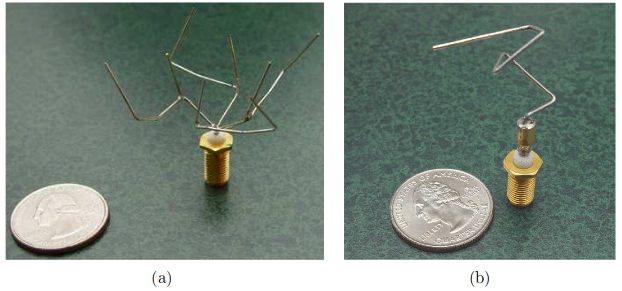
\includegraphics[scale=0.5]{img/nasa-antenne.png}
  \caption{Foto der Prototypen für unterschiedliche Anforderungen. \cite{AutomatedAntenna}}
  \label{fig:Ablauf_kurz}
\end{figure}


\subsection{GLEAM}
General Learning Evolutionary Algorthm and Method ist eine vom Kit entwickelte Methode um Aktionsketen zu berechnen. Dazu gehörtz zum beispiel das Aufeinandern abstimmen der Maschinen in einem Maschinenpark um so genannte totzeiten der Maschinen zu verringern also die gesamt auslastung zu erhöhen.

Mit GLEAM wurde auch versucht die Stuerung von 6-Achsigen Robotorarmen zu verbessern. Es konnte gezeigt werden das die Steuerung mit Gleam funktioniert, dies wurde aber leider nie der neue Industie Standart. Es wird immer noch mit der klasschischen xxxSteuerungxxx  gearbeitet. 


\subsection{Reainforcment learning with GA}
Reinforcment learning ist möglichweise einer der größten Anwendungsgebiete der GA. Hierbei werden Neuronale Netze nicht mit hilfe von Gradienstieg training, wie im Gundlagen Kapitel besprochen. Sondern mit hilfe von Genetischen Algorithmen. Dabei wird das Neuronale Netz nicht 




\subsection{Zusammenfassung}